\documentclass[10pt,a4paper,oneside,notitlepage]{report}
\usepackage[utf8]{inputenc}
\usepackage[english]{babel}
\usepackage{amsmath}
\usepackage{amsfonts}
\usepackage{amssymb}
\usepackage{hyperref}
\usepackage[table]{xcolor}  
\usepackage[margin=2.5cm]{geometry}
\usepackage{titling}
\usepackage{titlesec}
\usepackage{graphicx}
\usepackage{float}
\graphicspath{ {plots/} }

% kein einrücken bei neuen absätzen
\setlength{\parindent}{0pt}

% position titel
\setlength{\droptitle}{-2cm}

% abstand vor subsection titel
\titlespacing{\subsection}{0pt}{40pt}{8pt}

\author{Flurin Rindisbacher}
\title{How To Write Fast Numerical Code \\ \vspace{6 mm} \textbf{Assignment 1}}

\begin{document}
\maketitle

\section*{Exercise 1 - Get to know your machine}
I own a MacBook Pro (Retina, Mid 2012) 2.6 GHz Intel Core i7. According to \textit{sysctl -n machdep.cpu.brand\_string} and the Intel manuals the microarchitectural parameters are: \\

\begin{tabular}{|l|l|l|}
\hline 
\rowcolor{gray!30}
\textbf{Parameter} & \textbf{Value} & \textbf{Assignment} \\ 
\hline 
Processor manufacturer & Intel & a)\\ 
\hline 
Processor name & Core i7 & a)\\ 
\hline
Processor number & 3720QM  & a)\\ 
\hline
\# of cores & 4  & b) \\ 
\hline 
CPU-core frequency & 2.60GHz  & c)\\ 
\hline 
Tick/tok & It's a Tick model (Ivy Bridge, shrink to 22nm) & d) \\ 
\hline 
Cycles/issue for floating point additions & 1 add/cycle & e) \\ 
\hline 
Cycles/issue for floating point multiplications & 1 mul/cycle & f) \\ 
\hline 
Max. theoretical float peak performance & 2 flops/cycle and 5.2 Gflop/s & g) \\ 
\hline 
\end{tabular} 
\\
Source of Information:
\begin{itemize}
  \item \url{http://www.intel.com/content/dam/doc/manual/64-ia-32-architectures-optimization-manual.pdf} Page 2-37
  \item \url{http://ark.intel.com/products/64891/Intel-Core-i7-3720QM-Processor-6M-Cache-up-to-3_60-GHz}
  \item ``sysctl -n machdep.cpu.brand\_string''
\end{itemize}

\section*{Exercise 2 - Cost analysis}
\subsection*{a)}
let $C(N) = float\_muls(N) + float\_adds (N) + float\_divs(N) + float\_mins(N)$ with \\
$float\_muls = $ number of floating point multiplications \\
$float\_adds = $number of floating point additions \\
$float\_divs = $number of floating point divisions calls \\
$float\_mins = $number of floating point min() calls \\

\subsection*{b)}
There are two inner-most loops containing operations in the function \textit{strong\_closure}. Both of these for-loops are nested inside two other loops going from 0..N/2-1 and 0..N-1. Since both loops go from 0 to N-1 their bodies are executed: $N/2 * N * N = N^3/2$ times.
\\
$float\_divs = N^3/2$ \\
$float\_muls = 0$ \\
$float\_adds = 7*N^3/2$ \\
$float\_mins = 5*N^3/2$\\
and therefore $C(N) = N^3/2 float\_divs + 7*N^3/2 float\_adds + 5*N^3/2 float\_mins$ for the function strong\_closure()

\subsection*{c)}
I would define $C(N) = {\#flops}$. This would lead to a cost of $C(N) = 13*N^3/2 = 7.5*N^3$ for the strong\_closure() function.

\section*{Exercise 3 - Floyd Warshall}
\subsection*{a)}
There's nothing to document here...
\subsection*{b)}
The compute() function uses $2*N^3$ floating point operations (One addition and one comparison/min() call() per iteration) where $N$ is the number of nodes.
\subsection*{c)}
It turned out to be very hard to get consistent timing results. I'm working on a Mac OS X Yosemite which did not make the whole experience easier. First thing I had to do was disable Inte Turbo Boost using the Kernel Extension mentioned on the Lecture Website. Then there are other problem zones like "spotlight" randomly starting to index  documents when I'm timing my code... 

\subsubsection*{Compiler}
For all measurements gcc-4.9 (Homebrew gcc 4.9.2\_1) 4.9.2 \\
The argumnts for compiling fw.c were:\\
\begin{verbatim}
gcc-4.9 fw.c -o fw -O3 -mno-abm -fno-tree-vectorize
\end{verbatim}

\subsubsection*{Used timer}
In the end I decided to use the rdtsc method to measure the code. I wrote a small programm "find\_best\_timer.c" which after multiple tests with different input sizes lead me to believe that the rdtsc method gives me better results.

\subsection*{d)}
\subsection*{i)}
\begin{figure}[H]
\caption{Runtime plot fw.c}
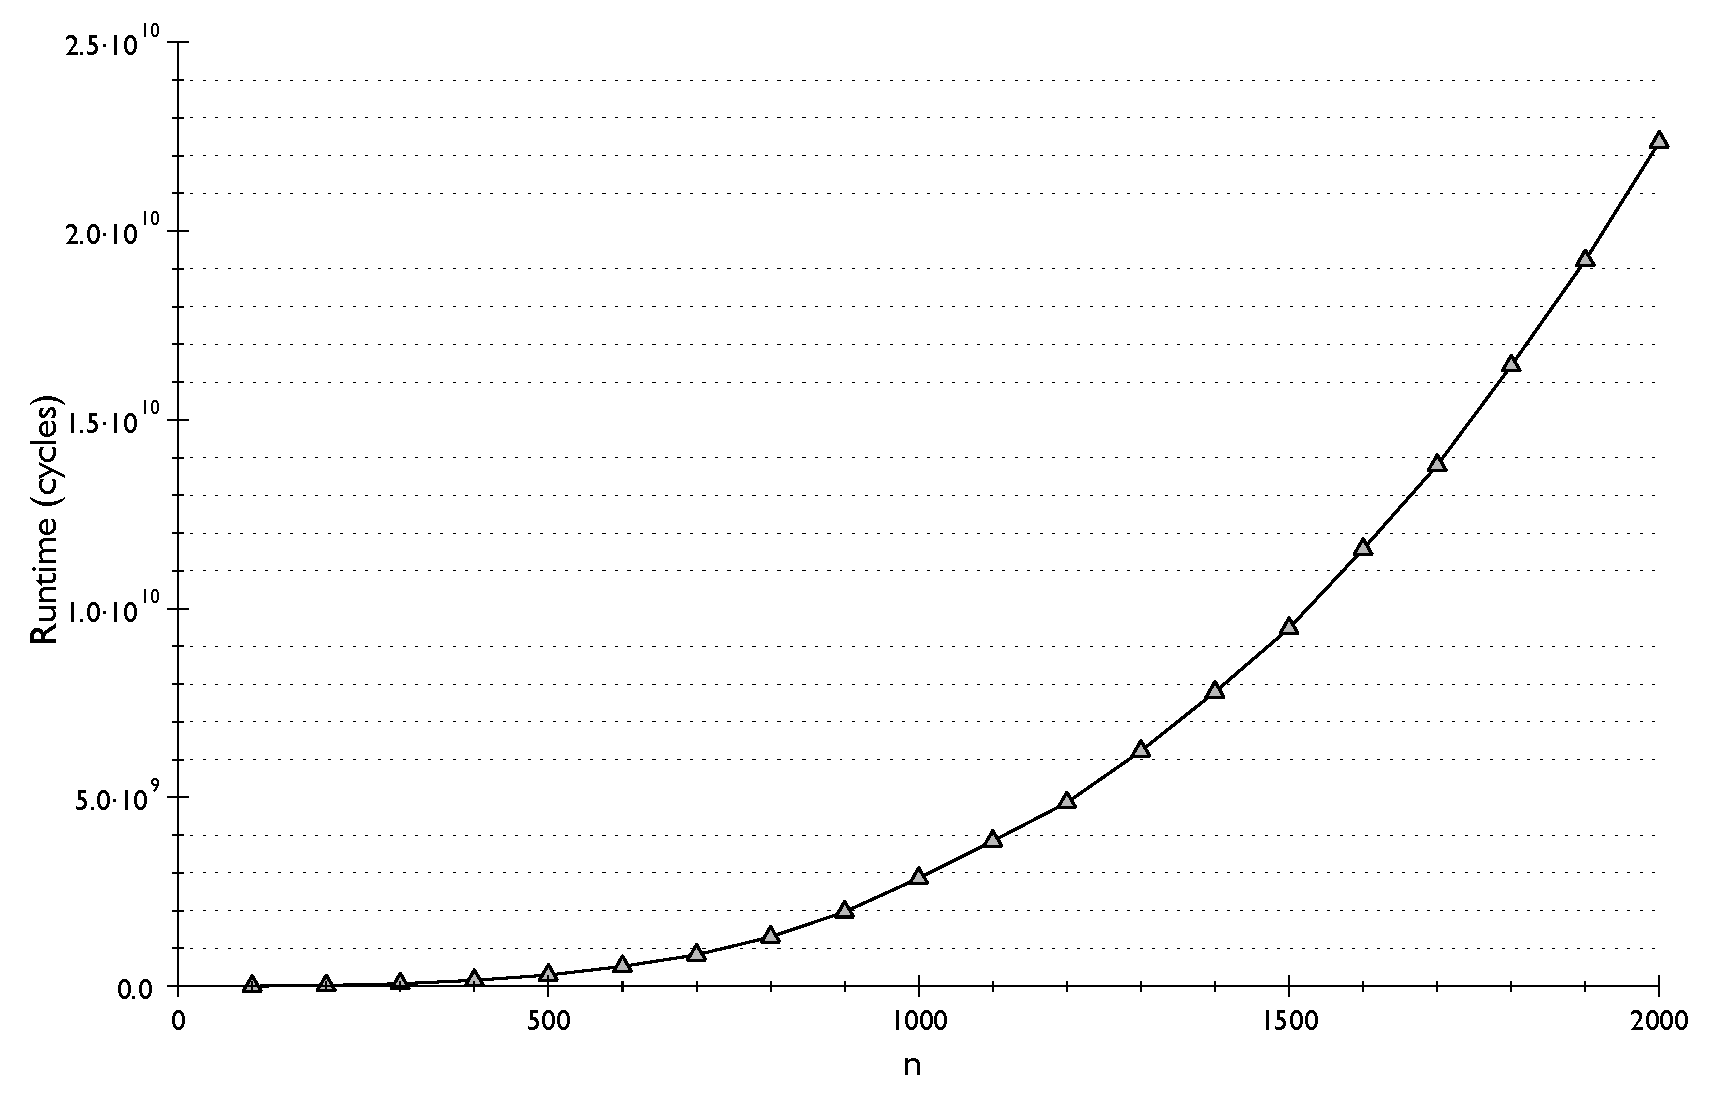
\includegraphics[height=9.5cm]{fw_runtime}
\end{figure}
\subsection*{ii)}
\begin{figure}[H]
\caption{Performance plot fw.c}
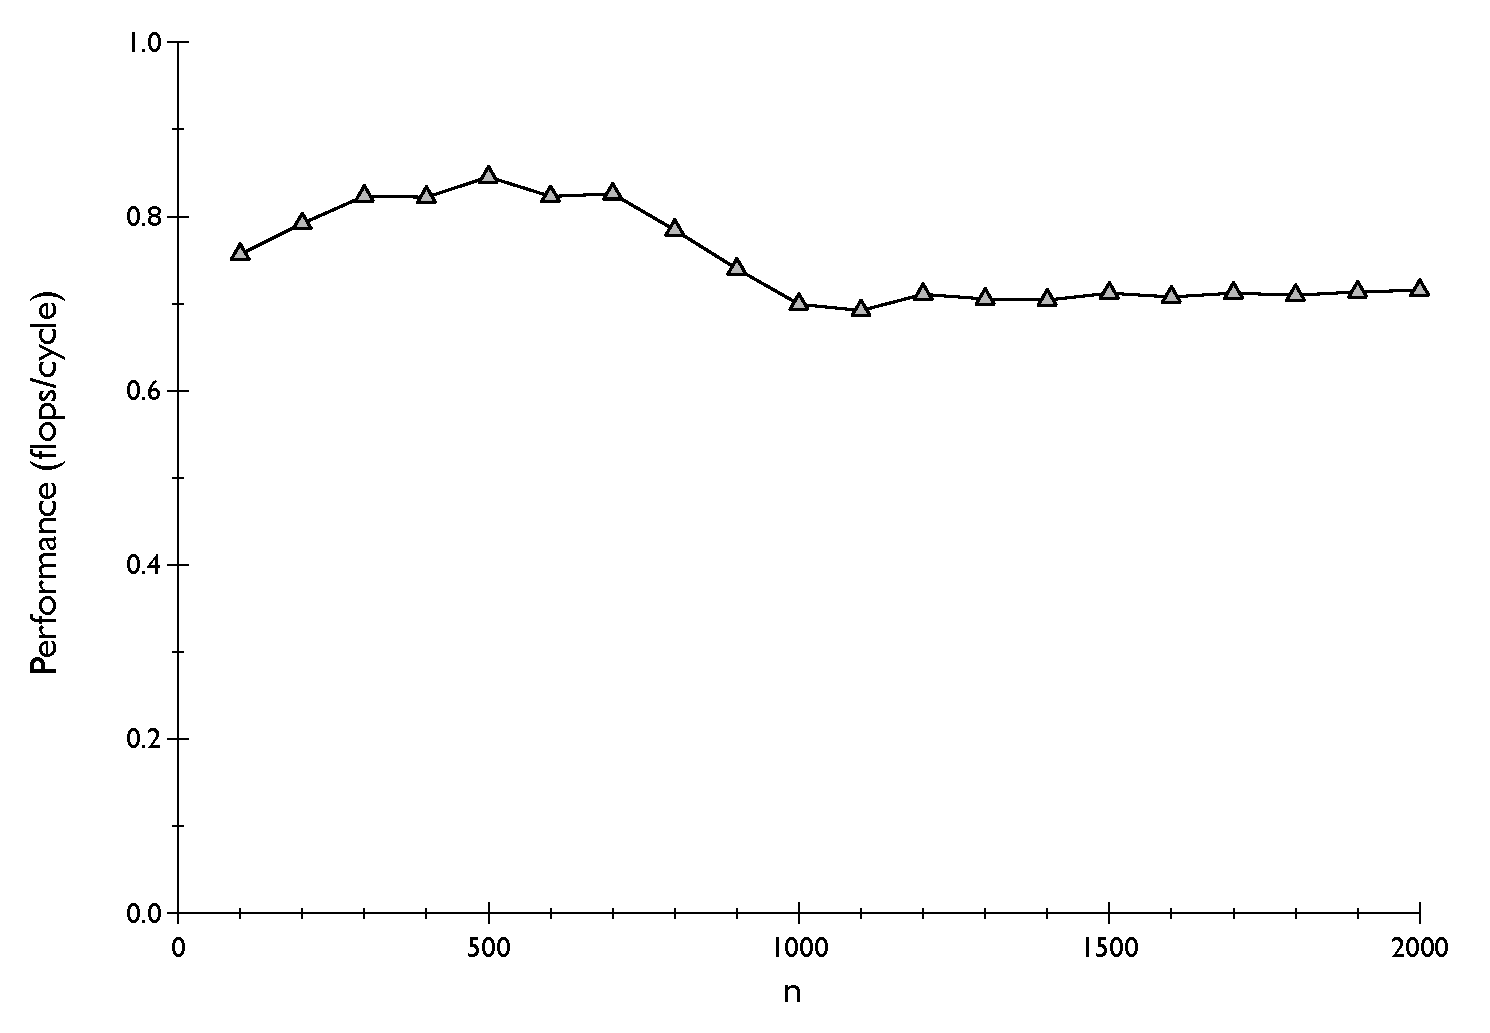
\includegraphics[height=9.5cm]{fw_performance}
\end{figure}
\subsection*{iii)}
\begin{figure}[H]
\caption{Percentage of the theoretical peak performance (2 flops/cycle) fw.c}
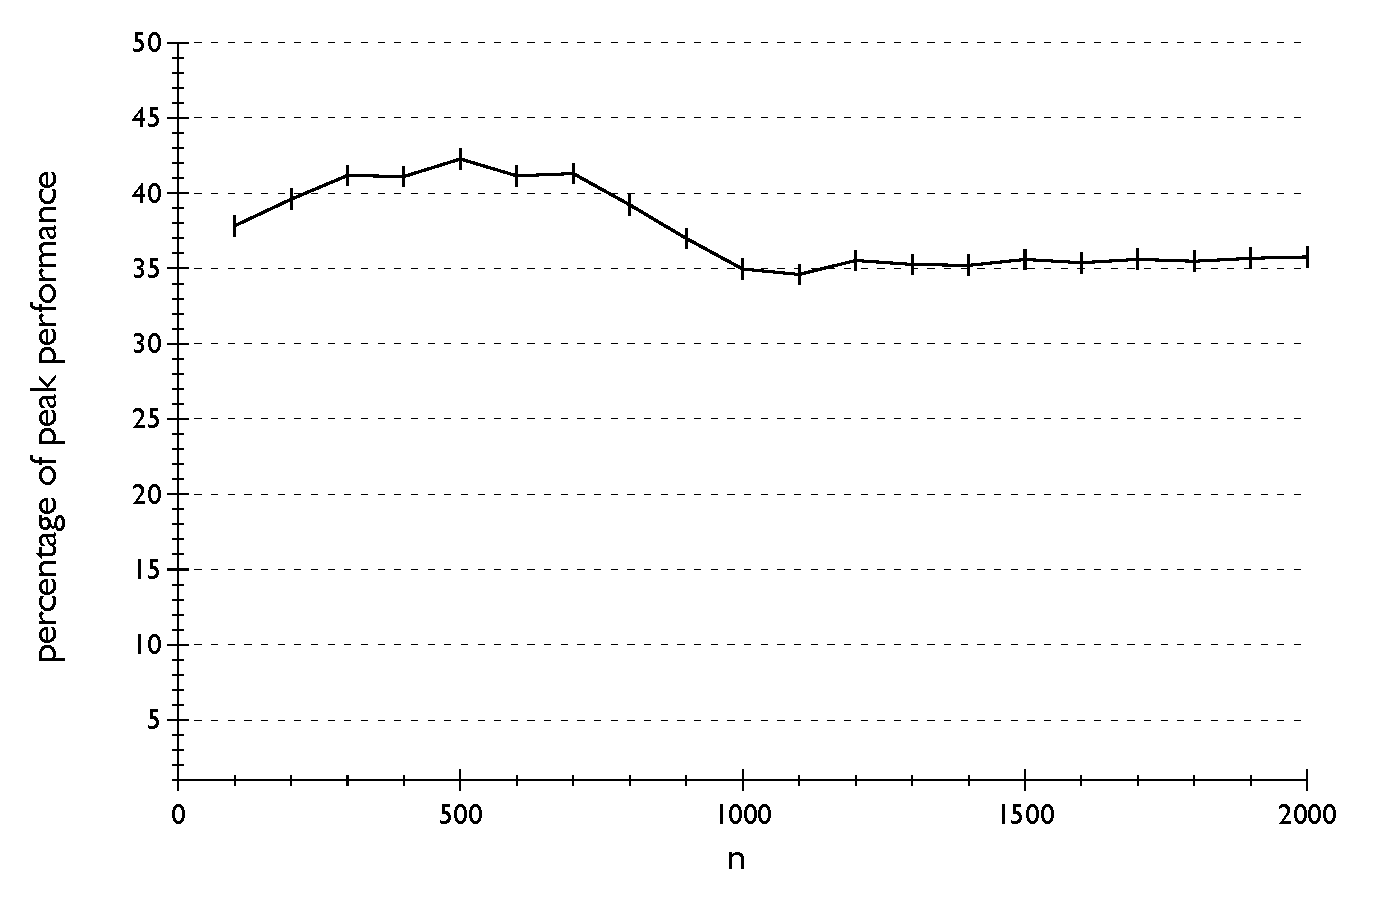
\includegraphics[height=9.5cm]{fw_percentage_of_peak}
\end{figure}
\subsection*{e)}
todo
\section*{Exercise 4 - Convex Combination}
\subsection*{a)}
Please see the file convex.c
\subsection*{b)}
See file convex.c. I used the rdtsc timing function.
\subsection*{c)}
\begin{figure}[H]
\caption{}
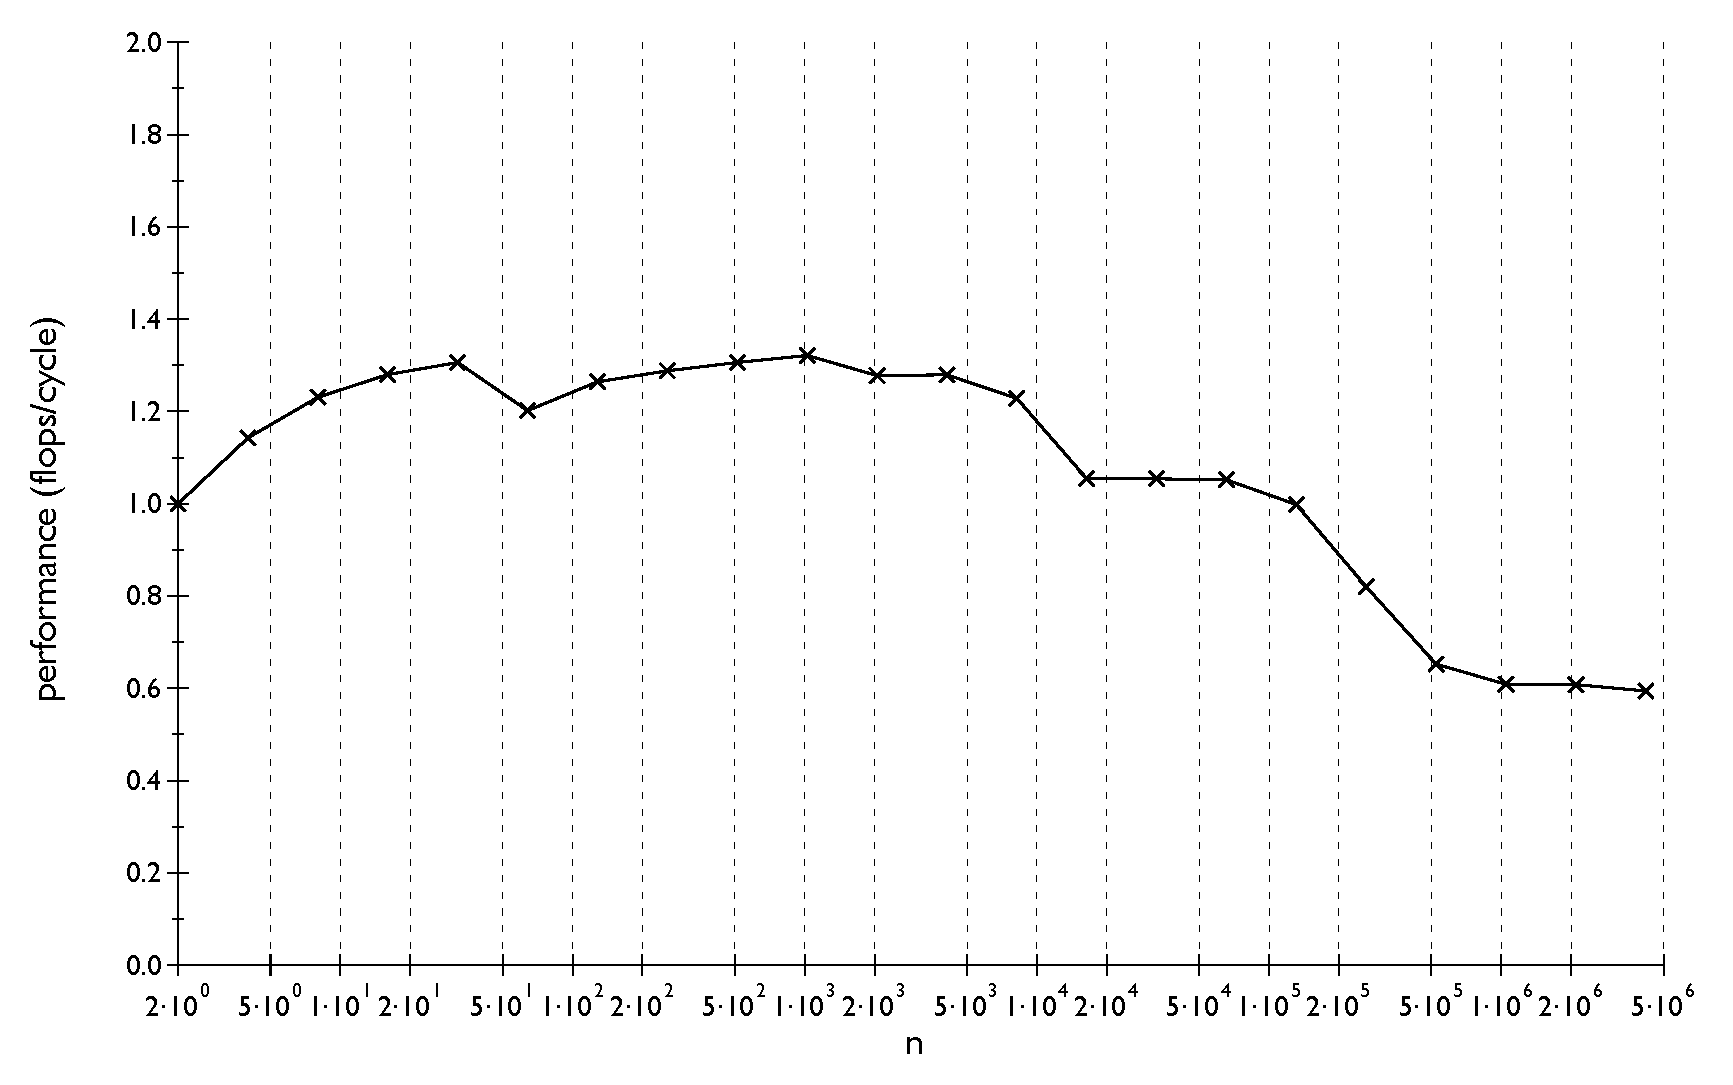
\includegraphics[height=9.5cm]{convex_performance}
\end{figure}
The convex combination costs $4*N$ floating point operations where $N$ is the size of the input arrays.
\subsection*{d)}
todo

\section*{Exercise 5 - Bounds}
\subsection*{a)}

\end{document}